
\documentclass{beamer}
%\documentclass[handout]{beamer}

\mode<handout>
{
  \usepackage{pgf}
  \usepackage{pgfpages}

\pgfpagesdeclarelayout{4 on 1 boxed}
{
  \edef\pgfpageoptionheight{\the\paperheight} 
  \edef\pgfpageoptionwidth{\the\paperwidth}
  \edef\pgfpageoptionborder{0pt}
}
{
  \pgfpagesphysicalpageoptions
  {%
    logical pages=4,%
    physical height=\pgfpageoptionheight,%
    physical width=\pgfpageoptionwidth%
  }
  \pgfpageslogicalpageoptions{1}
  {%
    border code=\pgfsetlinewidth{2pt}\pgfstroke,%
    border shrink=\pgfpageoptionborder,%
    resized width=.5\pgfphysicalwidth,%
    resized height=.5\pgfphysicalheight,%
    center=\pgfpoint{.25\pgfphysicalwidth}{.75\pgfphysicalheight}%
  }%
  \pgfpageslogicalpageoptions{2}
  {%
    border code=\pgfsetlinewidth{2pt}\pgfstroke,%
    border shrink=\pgfpageoptionborder,%
    resized width=.5\pgfphysicalwidth,%
    resized height=.5\pgfphysicalheight,%
    center=\pgfpoint{.75\pgfphysicalwidth}{.75\pgfphysicalheight}%
  }%
  \pgfpageslogicalpageoptions{3}
  {%
    border code=\pgfsetlinewidth{2pt}\pgfstroke,%
    border shrink=\pgfpageoptionborder,%
    resized width=.5\pgfphysicalwidth,%
    resized height=.5\pgfphysicalheight,%
    center=\pgfpoint{.25\pgfphysicalwidth}{.25\pgfphysicalheight}%
  }%
  \pgfpageslogicalpageoptions{4}
  {%
    border code=\pgfsetlinewidth{2pt}\pgfstroke,%
    border shrink=\pgfpageoptionborder,%
    resized width=.5\pgfphysicalwidth,%
    resized height=.5\pgfphysicalheight,%
    center=\pgfpoint{.75\pgfphysicalwidth}{.25\pgfphysicalheight}%
  }%
}


  \pgfpagesuselayout{4 on 1 boxed}[a4paper, border shrink=5mm, landscape]
  \nofiles
}
 % for handout 
%\setbeameroption{show notes} % uncomment to the the notes


\usepackage[T2A]{fontenc}
\usepackage[utf8]{inputenc}
\usepackage[english]{babel}
\usepackage{amssymb,amsfonts,amsmath,mathtext}
\usepackage{cite,enumerate,float,indentfirst}
\usepackage[dvips]{graphicx}
\usepackage[linesnumbered,ruled,vlined]{algorithm2e} % NEW
\usepackage{algorithmic}
\usepackage{listings}
\usepackage[square]{natbib}
\usepackage{multibib}

\definecolor{UniBlue}{RGB}{29,175,236}
%\setbeamercolor{title}{fg=UniBlue}
%\setbeamercolor{frametitle}{fg=UniBlue}
\setbeamercolor{structure}{fg=UniBlue}

\lstset{
        breaklines=true,
        basicstyle=\footnotesize\ttfamily,
        prebreak =\raisebox{0ex}[0ex][0ex]{\ensuremath{\hookleftarrow}},
        postbreak =\raisebox{0ex}[0ex][0ex]{\ensuremath{\hookleftarrow}}
}

\setbeamertemplate{footline}[page number]


\title[Text Analysis of Social Networks]{Text Analysis of Social Networks: \\ Working with FB.com and VK.com Data }
\subtitle{Seminar of CENTAL, Universit\'{e} catholique de Louvain, Louvain-la-Neuve, Belgium}
\author[Alexander Panchenko]{Alexander Panchenko \\ {\footnotesize \texttt{panchenko@lt.informatik.tu-darmstadt.de}}}

\institute{Language Technology Group, TU Darmstadt, Germany  }
\date{November 27, 2015}


\mode<presentation>
{
\usetheme{Luebeck}
\usecolortheme{default}
\useoutertheme{smoothbars}
}

\setbeamertemplate{navigation symbols}{}

\AtBeginSection[]
{
    \begin{frame}<beamer>
    \frametitle{Outline}
    \tableofcontents[currentsection] %,currentsubsection]
    \end{frame}
}



\setbeamercovered{transparent}
 
\begin{document}

\begin{frame}
  \titlepage
   \begin{figure}
    \centering
    %
\includegraphics[width=.3\textwidth]{fig/tu}
    %
\includegraphics[width=.2\textwidth]{fig/lt}
    \end{figure}
\end{frame}

\begin{frame}
 \setcounter{tocdepth}{1}
 \frametitle{Outline}
 \tableofcontents
 \setcounter{tocdepth}{2}
    
\end{frame}


%\frame{\titlepage}

\section[Data]{ Social Network Data }
\subsection{ }

\frame{
\frametitle{Acknowledgment: Digital Society Laboratory LLC}
 \begin{figure}
    \centering
    
\includegraphics[width=.8\textwidth]{fig/dsl}
    \end{figure}

\url{http://socialkey.ru/}
}

\frame {
\frametitle{Social networks from the users's standpoint}
 
 \textbf{Facebook (FB)} and \textbf{VKontakte (VK)}
\begin{figure}                         
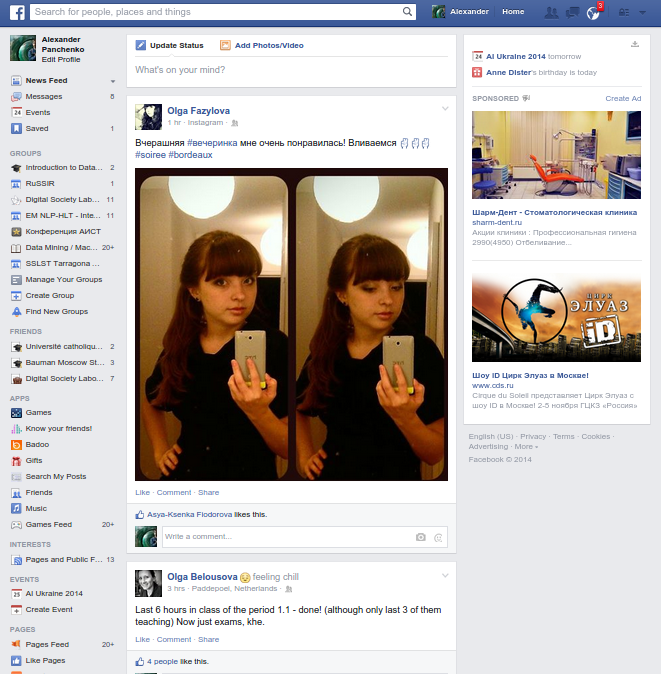
\includegraphics[width=0.5\textwidth]{fig/fb}
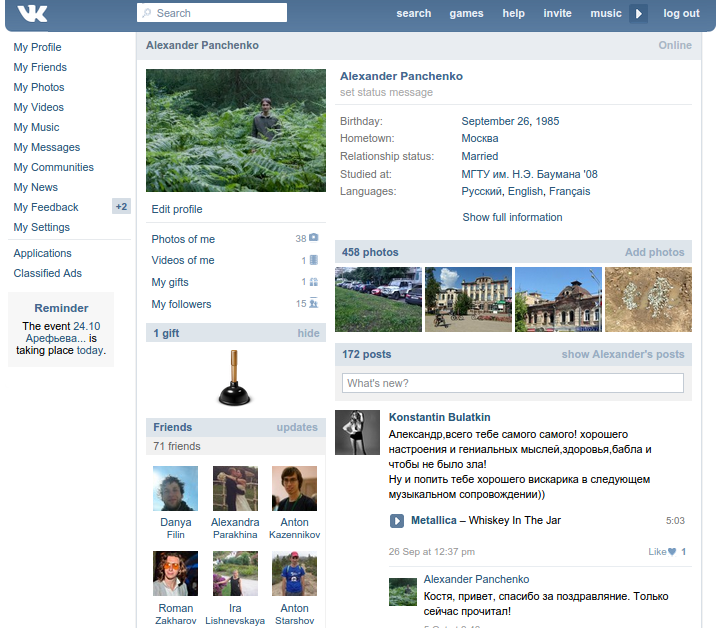
\includegraphics[width=0.5\textwidth]{fig/vk}

\end{figure}

}


\frame{
\frametitle{Social networks from the data miner's standpoint}


\textbf{Facebook (FB)} and \textbf{VKontakte (VK)}
 
\begin{itemize}
  \item \textbf{Profiles}: a set of user attributes
  \begin{itemize}
    \item categorical variables (region, city, profession, etc.)
    \item integer variables (age, graduation year, etc.)
    \item text variables (name, surname, etc.)
  \end{itemize}
  
  \item \textbf{Network}: a graph that relates users
  \begin{itemize}
    \item friendship graph
    \item followers graph
    \item commenting graph, etc.
  \end{itemize}
  
  \item \alert{\textbf{Texts}}:
  \begin{itemize}
  \item posts
  \item comments
  \item group titles and descriptions
  \end{itemize}
\end{itemize}

}


\frame{
\frametitle{Gathering of VK and FB data}

\begin{itemize}
  \item \alert{\textbf{Big Data}}: VK worth tens or even hundreds of TB
  \item \textbf{Decide} what do you need (posts, profiles, etc.).
  \item \textbf{Download}:
  \begin{itemize}
    \item API 
    \item Scraping
  \end{itemize}
  
  \item \textbf{Download limits} and \textbf{API limitations} are specific for each network.  

\item \textbf{Parallelization } is very practical, especially horizontal one:

\begin{itemize}
  \item Amazon EC2, Distributed Message Queues  

\begin{figure}                         
 %\includegraphics[width=0.5\textwidth]{fig/amazon}

\includegraphics[width=0.2\textwidth]{fig/nsq}

\includegraphics[width=0.3\textwidth]{fig/scala}
\end{figure}
\end{itemize}

\end{itemize}
}


\frame{
\frametitle{Storing VK and FB data }

\begin{itemize}
  \item Again, \alert{\textbf{Big Data}}
  \item \textbf{NoSQL} solutions are helpful
  \item \textbf{Raw data}: Amazon S3
  \item \textbf{For analysis}: HDFS 
  \item \textbf{Efficient retrieval}: Elastic Search
\begin{figure}                         
 %\includegraphics[width=0.5\textwidth]{fig/amazon}

\includegraphics[width=0.4\textwidth]{fig/hadoop}

\includegraphics[width=0.4\textwidth]{fig/es}
\end{figure}
\item 
  
\end{itemize}

}


\section[SNA]{ Social Network Analysis }
\subsection{}

\frame {
\frametitle{Social Network Analysis}

\begin{itemize}
  \item \textbf{Structure analysis}: friendship graph, comments graph, etc.
  \item \textbf{Content analysis:} profile attributes, posts, comments, etc. 
  \item \textbf{Combined approaches}.
    
\end{itemize}
  
\begin{block}{What scientific communities analyze social networks?}
\begin{itemize}
  \item 60s -- the first structural methods
  \item 00s -- online social network analysis boom
  \item \textbf{Social Network Analysis} community (Sociologists, Statisticians, Physicists)  
  \item \textbf{Data and Graph Mining} community
  \item \textbf{Natural Language Processing} community

\end{itemize}
\end{block}
 }
 
 
 \frame{
 \frametitle{Technologies for analysis of social networks}
 
 \begin{itemize}
   \item Machine Learning: \alert{\textbf{hidden vs observable}} user attributes
   \item \textbf{Training} of the model often can be scaled vertically

\begin{figure}                         

\includegraphics[width=0.25\textwidth]{fig/python}

\includegraphics[width=0.17\textwidth]{fig/scipy}

\includegraphics[width=0.25\textwidth]{fig/sklearn-logo}
\end{figure}


\item \textbf{Applying} the model should be scaled horizontally
   
\begin{figure}                         

\includegraphics[width=0.3\textwidth]{fig/hadoop}

\includegraphics[width=0.25\textwidth]{fig/spark}
\end{figure}
   
 \end{itemize}
 
 }

\section[User Gender]{ User Gender Detection}
\subsection{}

\frame {
 \frametitle{Problem}

\textit{Joint work with Andrey Teterin.}
 
 \begin{itemize}
  
 \item  \textbf{Detect gender of a user}
 \begin{itemize}
   \item to profile a user;
   \item user segmentation is helpful in search, advertisement, etc.
 \end{itemize}
 
 \item \textbf{By text written by a user}: 
 
 \begin{itemize}
   \item \cite{ciot2013gender}, \cite{koppel2002automatically}, \cite{goswami2009stylometric}, \cite{mukherjee2010improving}, \cite{peersman2011predicting}, \cite{rao2010classifying}, Rangel and Rosso~\cite{rangel2013use}, Al Zamal et al.\cite{al2012homophily} and Lui et al.~\cite{liu2012using}. 
 
\end{itemize}

 \item \alert{\textbf{By full name}}: \cite{burger2011discriminating}, Panchenko and Teterin [2014]

 
 \end{itemize}
 
 \textbf{}
}


\frame{

\frametitle{Online demo}

\url{http://research.digsolab.com/gender}

\begin{figure}                         
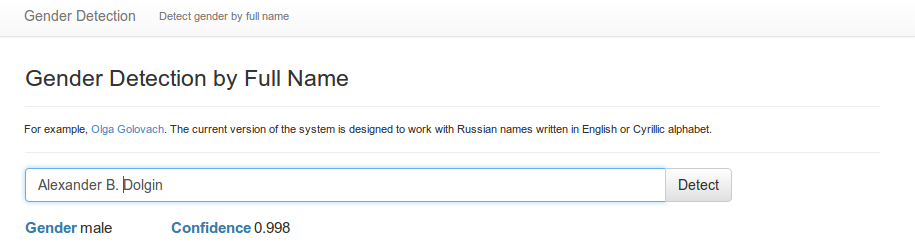
\includegraphics[width=1.0\textwidth]{fig/sample}
%\caption{Web interface.}
\end{figure}


\begin{figure}                         
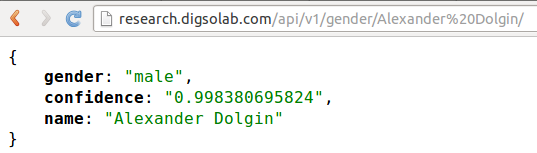
\includegraphics[width=0.7\textwidth]{fig/api}
%\caption{RESTful API interface.}
\end{figure}

 }


\frame{
\frametitle{Training Data}

\begin{itemize}

\item \alert{100,000 full names} of Facebook users with known gender 

\item \alert{full name} -- first and last name of a user 
\item \alert{gender}: male or female

\item names written in both Cyrillic and Latin alphabets

\item ``Alexander Ivanov'', ``Masha Sidorova'', ``Pavel Nikolenko'', etc.
 
\end{itemize}
}


\frame {
\frametitle{Training Data}
 
\begin{figure}
\centering
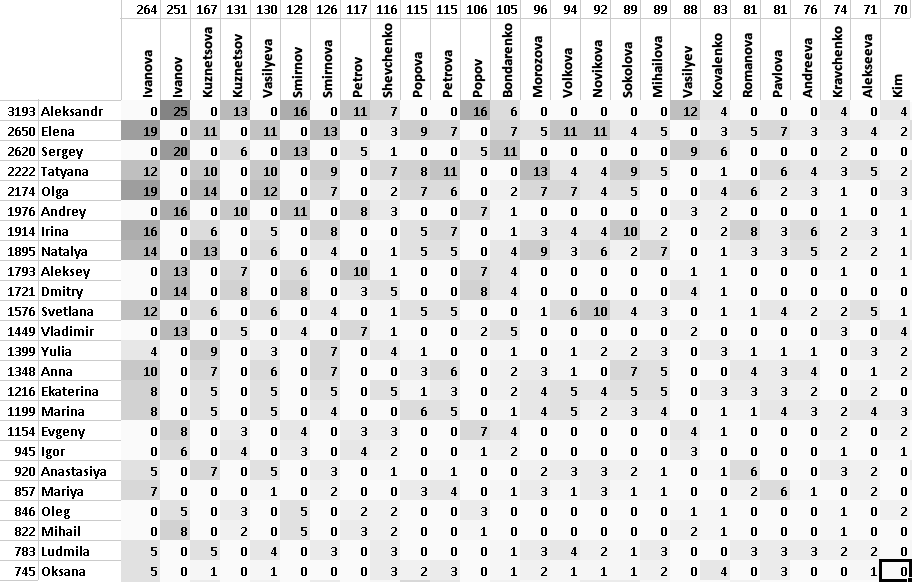
\includegraphics[width=1.0\textwidth]{fig/matrix3} 
\caption{ Name-surname co-occurrences: rows and columns are sorted by frequency. }
\end{figure}

}


\frame{\frametitle{Character endings of Russian names}

\begin{itemize}
\item \alert{72\%} of first names have typical male/female ending
\item \alert{68\%} of surnames  have typical male/female ending
\item a \alert{typical male/female ending} splits males from females with an error less than 5\%

\item gender of $\geq$ \alert{50\%} first names recognized with \alert{{8 endings}}

\item gender of $\geq$ \alert{50\%} second names recognized with \alert{{5 endings}}

\begin{block}{Conclusion}
Simple symbolic ending-based method cannot robustly classify about \alert{30\% of names}. This motivates the need for a more sophisticated statistical approach. 
\end{block}

\end{itemize}
}

\frame{
\frametitle{Character endings of Russian names}


\begin{table}[h]

\footnotesize

\begin{center}
\begin{tabular}{|l|ll|l|l|l|l|}
\hline
\bf Type & \bf Ending & & \bf Gender & \bf Error, \% &  \bf Example \\ \hline \hline

first name & na & (\textcyr{на}) & female & 0.27 & Ekateri\textbf{na} \\
first name & iya & (\textcyr{ия}) & female & 0.32 & Anastas\textbf{iya} \\
first name & ei & (\textcyr{ей}) &  male & 0.16 & Serg\textbf{ei} \\
first name & dr & (\textcyr{др}) & male & 0.00 & Alexan\textbf{dr} \\
first name & ga & (\textcyr{га}) & male & 4.94 & Sere\textbf{ga} \\
first name & an  & (\textcyr{ан}) & male & 4.99 & Iv\textbf{an} \\
first name & la & (\textcyr{ла}) & female & 4.23 & Luidmi\textbf{la} \\
first name & ii & (\textcyr{ий}) & male & 0.34 & Yur\textbf{ii} \\
second name & va & (\textcyr{ва})  & female & 0.28 & Morozo\textbf{va} \\
second name & ov & (\textcyr{ов})  & male & 0.21 & Objedk\textbf{ov} \\
second name & na & (\textcyr{на})  & female & 2.22 & Matyushi\textbf{na} \\
second name & ev & (\textcyr{ев}) & male & 0.44 & Serge\textbf{ev} \\
second name & in & (\textcyr{ин}) & male & 1.94 & Teter\textbf{in} \\
 
\hline
\end{tabular}
\end{center}
\caption{ Most discriminative and frequent two character endings of Russian names.  }
\label{tab:endings}
\end{table}
}


\frame{
\frametitle{Gender Detection Method}

\begin{itemize}
\item \alert{input}: a string representing a name of a person
\item \alert{output}:  gender (male or female)
\item binary classification task

\end{itemize}

\begin{block}{Features}

\begin{itemize}
\item endings
\item character $n$-grams
\item dictionary of male/female names and surnames
\end{itemize} 
\end{block}

\begin{block}{Model}
\begin{itemize}
  \item L2-regularized Logistic Regression
\end{itemize}
\end{block}


}


\frame{
\frametitle{Features}

\begin{block}{Character $n$-grams}
\begin{itemize}
%  \item $k$ most frequent unigrams, bigrams, trigrams 
\item males: Alexander Yaroskavski, Oleg Arbuzov
\item females: Alexandr\textbf{a} Yaroskavska\textbf{ya}, Nayali\textbf{ya} Arbuzov\textbf{a}
\item BUT: ``Sidorenko'', ``Moroz'' or ``Bondar''!   
\item two most common one-character endings: ``a'' and ``ya'' (``\textcyr{я}'')
 
\end{itemize}
\end{block}

\begin{block}{Dictionaries of first and last names}

\begin{itemize}

\item probability that it belongs to the male gender: $P(c=male|firstname)$, $P(c=male|lastname)$.

%$$ P(c=male|w) = \frac{n_{male}^w }{\sum_{c \in \{male, female\}} n_{c}^w},$$

%\item $n_{male}^w$ --  number of male profiles with the first/last name $w$ in the dictionary

%\item probability that first name is of male gender $P(c=male|firstname)$
%\item probability that the last name is of male gender $P(c=male|lastname)$
\item 3,427 first names, 11,411 last names

\end{itemize}
\end{block}
 
}


%\frame{
%\frametitle{Model}

%\begin{itemize}
%  \item L2-regularized Logistic Regression
%\item yields reasonable results for the NLP-related problems

%\item model $\mathbf{w}$, feature vector $\mathbf{x}$
%\item classification:
%$$
%P(y=1|\mathbf{x}) = \frac{1}{1 + e^{-\mathbf{w}^T \mathbf{x}}  }.
%$$
%\end{itemize}
%}


\frame{
\frametitle{Results}



\begin{table}[h]

\tiny

\begin{center}
\begin{tabular}{|l|l|l|l|l|}
\hline
\bf Model & \bf Accuracy & \bf Precision & \bf Recall & \bf F-measure \\ \hline \hline

\textit{rule-based baseline} &  0,638 & \bf 0,995 & 0,633 & 0,774 \\   

\textit{endings} & 0,850 $\pm$ 0,002 & 0,921 $\pm$ 0,003 & 0,784 $\pm$ 0,004 & 0,847 $\pm$ 0,002 \\

\textit{3-grams} & 0,944 $\pm$ 0,003 & 0,948 $\pm$ 0,003 & 0,946 $\pm$ 0,003 & 0,947 $\pm$ 0,003 \\

\textit{dicts} & 0,956 $\pm$ 0,002 & \bf 0,992 $\pm$ 0,001 & 0,925 $\pm$ 0,003 & 0,957 $\pm$ 0,002 \\ 

\textit{endings+3-grams} & 0,946 $\pm$ 0,003 & 0,950 $\pm$ 0,002 & 0,947 $\pm$ 0,004 & 0,949 $\pm$ 0,003 \\

\textit{3-grams+dicts} & 0,956 $\pm$ 0,003 & 0,960 $\pm$ 0,003 &  0,957 $\pm$ 0,004 &  0,959 $\pm$ 0,003 \\ 
 
\textit{endings+3-grams+dicts} & \bf 0,957 $\pm$ 0,003 & 0,961 $\pm$ 0,003 & \bf 0,959 $\pm$ 0,004 & \bf 0,960 $\pm$ 0,002  \\

\hline
\end{tabular}
\end{center}
\caption{ Results of the experiments on the training set of 10,000 names. Here \textit{endings} -- 4  Russian female endings, \textit{trigrams} -- 1000 most frequent 3-grams, \textit{dictionary} -- name/surname dict. This table presents precision, recall and F-measure of the female class. }
\label{tab:results}
\end{table}

}


\frame{
\frametitle{Results}

\begin{figure}
    \centering
    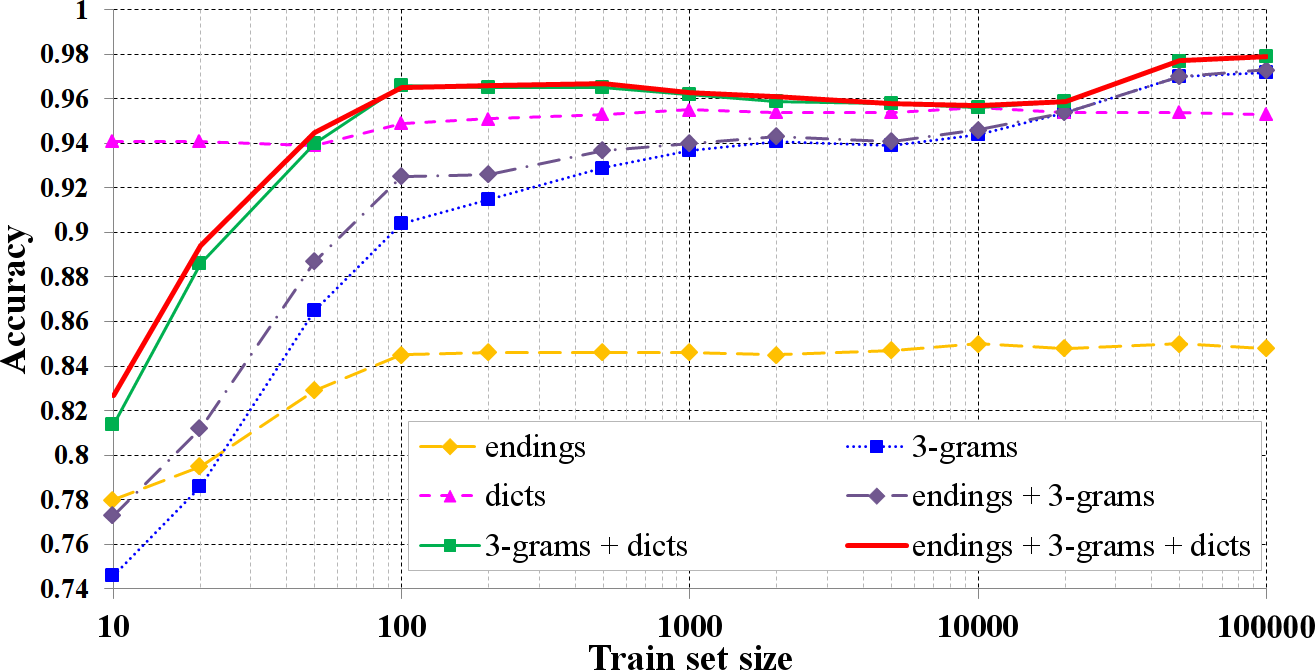
\includegraphics[width=1.0\textwidth]{fig/lc-all} 
    \caption{ Learning curves of single and combined models. Accuracy was estimated on separate sample of 10,000 names.  }
    \label{fig:curve}
\end{figure}

}


\frame{
\frametitle{Results}

\begin{figure}
\centering
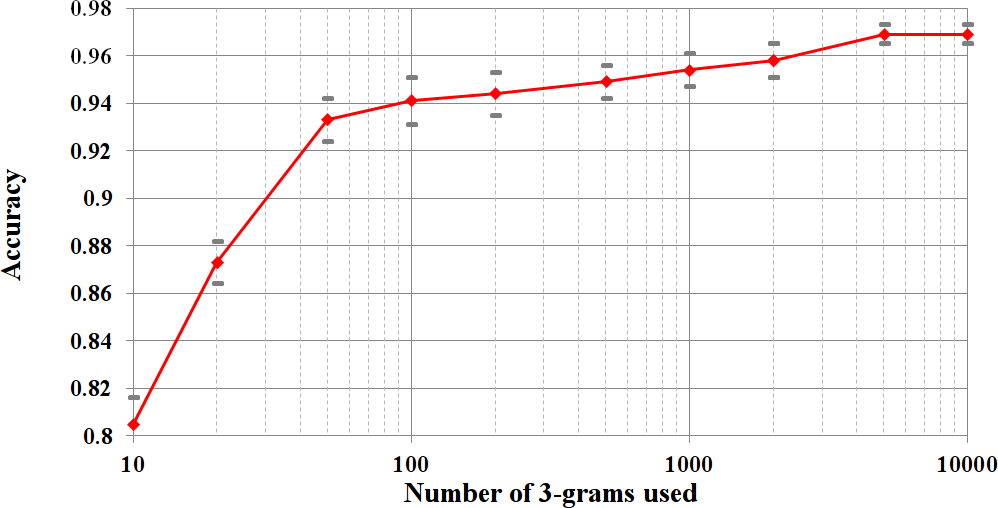
\includegraphics[width=1.0\textwidth]{fig/ngrams} 
\caption{ Accuracy of the model \textit{3-grams} function of the number of features used $k$. }
\label{fig:ngrams}
\end{figure}
}



\frame{
\frametitle{Error Analysis}

There are several types of errors: 

\begin{itemize}
\item Inconsistent annotation, such as ``Anna Kryukova (male)'' or ``Boris Krolchansky (female)''. 
\item Name string is neither male nor female, but rather a name of a group, e.g. ``Wikom Tools'', ``Kazakh University of Humanities'' or ``Privat Bank''.

\item Name string represents a foreign name, e.g. ``Abdulloh Ibn Abdulloh'', ``Brooke Alisson'', ``Ulpetay Niyetbay'' or ``Yola Dolson''. Our model was not trained to deal with such names. 

\item Meaningless or partially anonymized names names, e.g. ``Crazzy Ma'', ``Un Petit Diable'', ``Vv Tt'', ``Vio La Tor'' or ``Muu Muu''. Additional information is required to derive gender of such users.

\item People with rare names or surnames, e.g. ``Guldjan Reyzova'',  ``Yagun Zumpelich'' or ``Akob Saakan''. These are people with common names and surnames in other countries, such as Georgia, Kazakhstan, Azerbaijan or Tajikistan. In our dataset, people from these countries are under-represented. 

\item Full names that can denote both males and females, e.g. ``Jenya Chekulenko'', ``Jenya Sergienko'', ``Sasha Sidorenko'' or ``Sasha Radchenko''. Additional information is required to infer gender of such people.

\item Misclassifications of common names, e.g. ``Ilya Nasorshin'', ``Oleg Dubovik'' or ``Elena Antropova''. 
\end{itemize}
}


\frame{
\frametitle{Error Analysis}
\begin{table}[h]
\tiny
\begin{center}
\begin{tabular}{|l|ll|ll|}
\hline
 &  \bf Train Set Errors &  & \bf Test Set Errors & \\ \hline 
 &  \bf name & \bf true class & \bf name & \bf true class \\ \hline \hline
1 & Lea Shraiber  & female & Ilya Nadorshin & male \\  
2 & Profanum Vulgus  & female & Rustem Saledinov & male \\  
3 & Anna Kryukova & male & Erkin Bahlamet & male \\  
4 & Gin Amaya & male & Gocha Lapachi & male \\  
5 & Gertrud Gallet  & female & Muttaqiyyah Abdulvahhab & female \\  
6 & Dolores Laughter & female & Yola Dolson & female \\  
7 & Di Nolik  & male & Heiran Gasanova & female \\  
8 & Jūlija Hotiņeca  & female & Hadji Murad & male \\  
9 & Gic Globmedic  & female & Jenya Chekulenko & female \\  
10 & Ulpetay Niyetbay  & female & Tury.Ru Domodedovskaya Metro Office & male \\  
11 & Olga Shoff  & male & Elmira Nabizade & female \\  
12 & Phil Golosoun  & male & Niko Liparteliani & male \\  
13 & Tsitsino Shurgaya & female & Oleg Grin' & male \\  
14 & Anna Grobov  & female & Santi Zarovneva & female \\  
15 & Linguini Incident & female & Misha Badali & male \\  
16 & Toma Oganesyan & female & Che Serega & male \\  
17 & Swon Swetik & female & Petr Kiyashko & male \\  
18 & Adel Simon & female & Sandugash Botabaeva & female \\  
19 & Ant Kam-  & male & Jenya Sergienko & female \\  
20 & Xristi Xitrozver  & female & Abdulloh Ibn Abdulloh & female \\  
21 & Anii Reznookova  & female & Naikaita Laitvainenko & male \\  
22 & Aurelia Grishko & male & Fil Kalnitskiy & male \\  
23 & Alex Bu  & female & Helen Hovel' & female \\  
24 & Karen Karine & female & Valery Kotelnikov & male \\  
25 & Russian Spain & female & Max Od & male \\  
26 & Lucy Walter & male & Jean Kvartshelia & male \\  
27 & Aysah Ahmed & female & Adjedo Trupachuli & female \\  
28 & Kiti Iz  & female & Ainur Serikova & female \\  
29 & Cutejilian Juka  & female & Privat Bank & female \\  
30 & Azer Dunja  & male & No Limit & female \\  
\hline
\end{tabular}
\end{center}
\caption{ Examples of train and test set errors of the model \textit{endings+3-grams+dicts}. Here Cyrillic characters were transliterated into English in the standard way. }
\label{tab:errors}
\end{table}
}



\section[User Language]{ User Language Detection }
\subsection{}

\frame{
\frametitle{ Problem }


\begin{block}{Motivation}
\begin{itemize}
\item Goal: to detect \alert{Russian-speaking users}
\item Cyrillic alphabet is used also by Ukrainian, Belorussian, Bulgarian, Serbian, Macedonian, Kazakh, etc
\end{itemize}
\end{block}


\begin{block}{Research Questions}
\begin{itemize}
\item Which method is the best for Russian language?
\item How to adopt it to the FB profile?
\end{itemize}
\end{block}


\begin{block}{Contributions}

\begin{itemize}
\item Comparison of Russian-enabled language detection modules.
\item A technique for identification of Russian-speaking users.
\end{itemize}
\end{block}

}


\frame{
\frametitle{Method}

\begin{itemize}
  \item \alert{input:} a FB user profile
  \item \alert{output:} is Russian-speaker?  (or a set of languages user speaks)
\end{itemize}

\begin{block}{Common Russian character trigrams}
"на ", " пр", " то", " не", " ли", " по", "но ", " в ", " на", " ть", " не", " и ",  " ко", " ом", "про", "то ", " их",  " ка", "ать", "ото", " за", " ие", "ова", "тел", "тор",  " де", "ой ", "сти", " от", "ах ", " ми", "стр",  " бе", " во", " ра", "ая ", "ват", "ей ", "ет ", " же", "иче", "ия ", "ов ", "сто", " об", "вер", "го ",  "и в", "и п", "и с", "ии ", "ист", "о в", "ост", "тра", " те", "ели", "ере", "кот", "льн", "ник", "нти", "о с"

\end{block}

}


\frame{
\frametitle{Existing modules for language identification}

\begin{itemize}
\item \textbf{langid.py}
    \begin{itemize}
    \item \url{https://github.com/saffsd/langid.py}
    \item Advanced n-gram selection
    \end{itemize}

\item \textbf{chromium compact language detector (cld)}
    \begin{itemize}
    \item https://code.google.com/p/chromium-compact-language-detector
    \end{itemize}
    
\item \textbf{guess-language} 

    \begin{itemize}
    \item \url{https://code.google.com/p/guess-language}
    \end{itemize}
    
\item \textbf{Google Translate API}

    \begin{itemize}
    \item \url{https://developers.google.com/translate/v2/using_rest#detect-language}
    \item 20\$/1M characters
    \end{itemize}
    
    
\item \textbf{Yandex Translate API} 
    \begin{itemize}
    \item \url{http://api.yandex.ru/translate}
    \item Free of charge, 1M of characters / day (by September 2013)
    \end{itemize}
    
\item \alert{\textbf{Many more}}, e.g. \texttt{language-detection} for Java
\end{itemize}
}


\frame{
\frametitle{DBpedia Dataset}

\begin{figure}
    \centering
    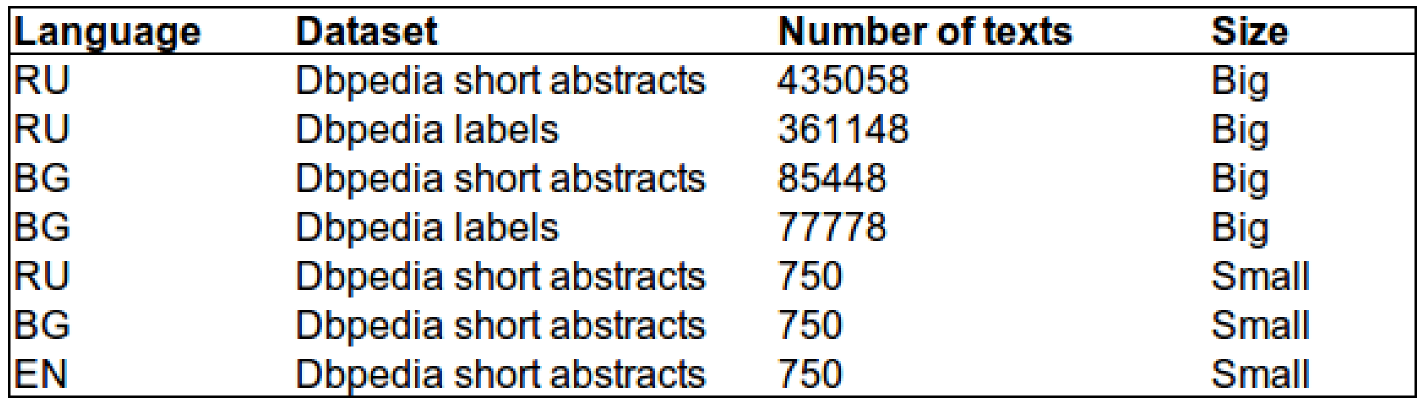
\includegraphics[width=1.0\textwidth]{fig/dbpedia} 
\end{figure}

}


\frame{
\frametitle{Accuracy of Different Language Detection Modules}

\begin{figure}
    \centering
    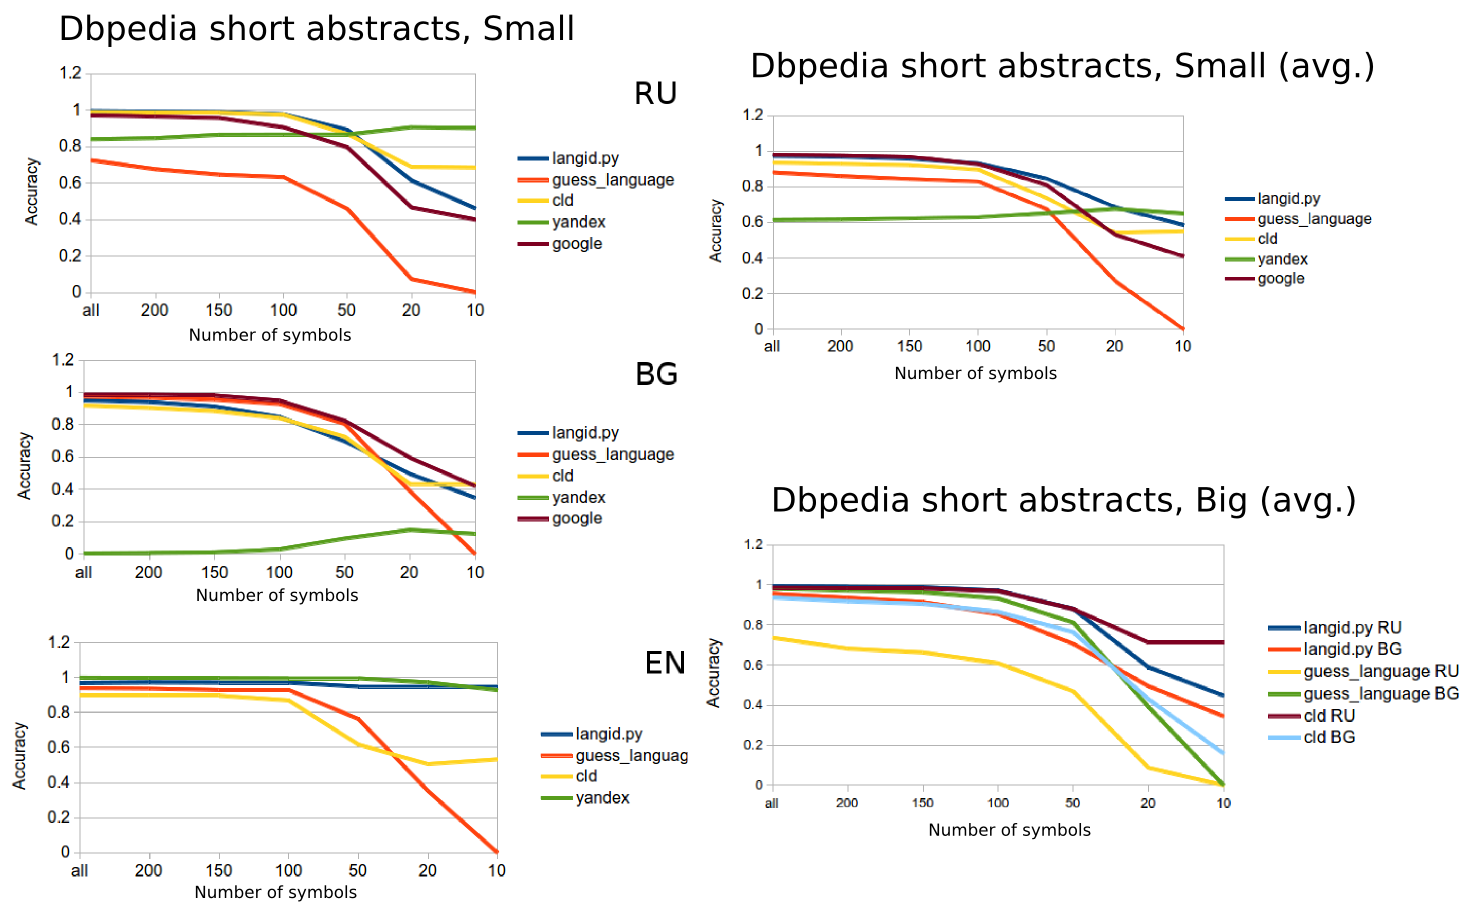
\includegraphics[width=1.0\textwidth]{fig/ld-results} 
\end{figure}
}

\frame{
\frametitle{Facebook Dataset: Method}

%\begin{block}{Method }

\begin{itemize}
\item \textbf{Profile text}: posts + comments + user names -- Latin symbols.

\item \textbf{Profile text length}: 3,367 +- 17,540   
\item \textbf{Russian-speakers}: P(ru) > 0.95
\item \textbf{Core Russian-speakers}:
\begin{itemize} 
 \item P(ru) > 0.95
 \item  \# Cyrillic symbols >= 20\% 
 \item locale is  \texttt{ru\_RU}
\end{itemize}

\end{itemize}
%\end{block}

}

\frame{
\frametitle{Facebook Dataset: Results}


\begin{itemize}
\item \textbf{9,906,524} public FB profiles (>= 50 cyr. characters)
\item 8,687,915 \textbf{(88\%)} Russian-speaking users 
\item 3,190,813 \textbf{(32\%)} core Russian-speaking public Facebook users
\item 5,365,691 \textbf{(54\%)} of profiles with no profile text (<= 200 characters)
\end{itemize}


} 


\section[User Interests]{User Interests Detection}
\subsection{}

\frame{
\frametitle{Problem}


\textit{Joint work with Dmitry Babaev and Sergei Objedkov.}

\begin{itemize}
  \item \textbf{\alert{input}}: \textit{some} SN data representing a user
  \item \textbf{\alert{output}}: list of user interests
\end{itemize}


\begin{block}{Motivation}
\begin{itemize}
  \item \alert{Advertisement}: targeting, user segmentation, etc. 
  \item Recommendations of content and friends
  \item Customization of user experience
  \item \ldots
\end{itemize}
\end{block}
}


\frame{
\frametitle{ Data: FB and VK groups }

\begin{block}{Text corpus}
\begin{itemize}
  \item 41 million of VK groups
  \item 11 million of FB publics
  \item 1.5 million of FB groups
\end{itemize}
\end{block}

\begin{block}{Data format}
\begin{itemize}
  \item Title and/or description
  \item List of members
  \item Number of comments, likes, posts by a member
\end{itemize}
\end{block}

}




\frame{
\frametitle{ Data: VK groups }

\begin{figure}
    \centering
    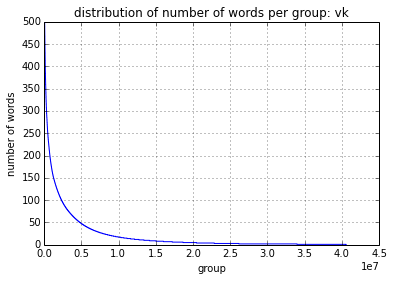
\includegraphics[width=0.48\textwidth]{fig/number-of-words-per-group} 
    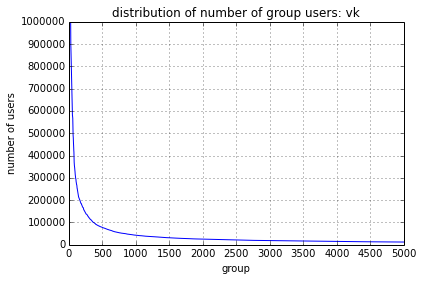
\includegraphics[width=0.52\textwidth]{fig/num} 
\end{figure}
}



\frame{
\frametitle{ 253 interests detected by our system }

\begin{figure}
    \centering
    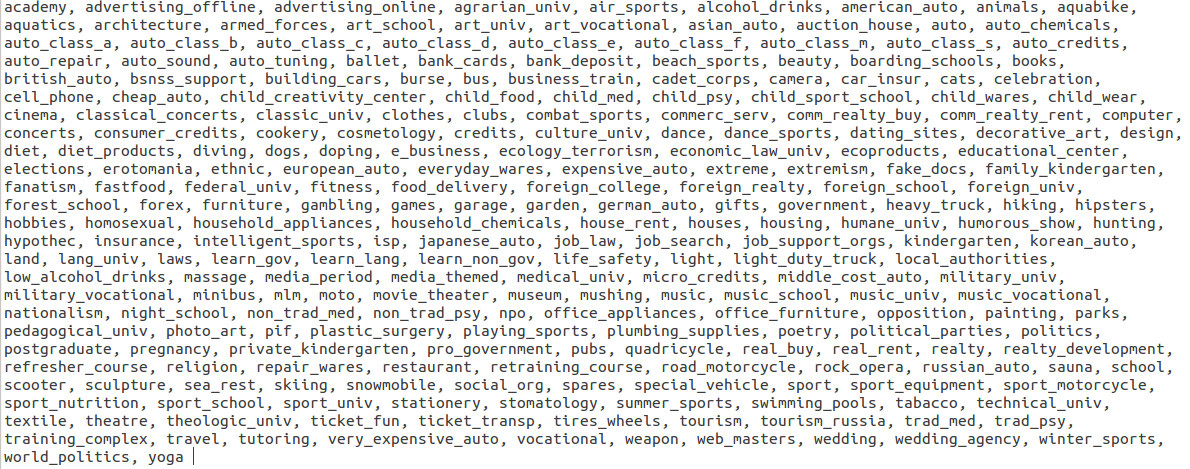
\includegraphics[width=1.05\textwidth]{fig/t-cats} 
\end{figure}
}


\frame{
\frametitle{Method}

\begin{enumerate}
  \item Create a text index of groups
  \item Create a keyword list for each of 253 interests
  \item \textbf{KW classifier}:
  \begin{itemize}
    \item Retrieve top $k$ groups retrieved by a set interest keywords
    \item Rank by TF-IDF
    \item Associate group's interests with its users
    \item A group may have multiple interests
  \end{itemize}
  
  \item \textbf{ML classifier:}
  \begin{itemize}
    \item Use top $k$ groups as a training data
    \item BOW features
    \item Keyword features
    \item Linear models: L2 LR, Liner SVM, NB
    \item Classify all groups
    \item A group may have up to three top interests
    \item Associate group's interests with its users
  \end{itemize}
\end{enumerate}
}


\frame{
\frametitle{Association of group's interests with its users}

\textbf{Engagement of a person into an interest category} is proportional to the activity of the person in groups of this category:

$$
e  \approx w_{like} \cdot l + w_{s.comm} \cdot cs + w_{l.comm} \cdot cl + w_{repost} \cdot r 
$$

\begin{itemize}
\item $l$ -- the number of post likes
\item $cs$ -- the number of short comments
\item $cl$ -- the number of long comments
\item $r$ -- the number of reposts
\end{itemize}


%$w_{likes} = \frac{1}{18}, w_{repost} = \frac{1}{3}, w_{s.comm} = \frac{1}{2}, w_{l.comm} = \frac{1}{1}.$

%The engagement is normalized by the 95-th percentile:

%$$
%N_m(x) =\left\{
%    \begin{array}{ll}
%        1 & \text{ if } x \ge p_x \\
%        \frac{x}{p_m} &  \text{ if } x < p_x 
%    \end{array}
%    \right,
%$$

%where $p_m -$ is the $m$-th percentile.  

%Therefore, engagement of a user $e$ to a category ranges from 0 to 1. Yet, 1 may mean different absolute number of actions (likes, reposts and so on), depending on the average activity per category.

\textbf{Association score of a user and an interest} depends on engagement in a group and on the number of groups:

$$all \approx  \alpha \cdot e_{fb} \cdot g_{fb} +  \beta \cdot e_{vk} \cdot g_{vk} .$$ 

\begin{itemize}
\item $e_{vk}$, $e_{fb}$  -- engagement into VK/FB interest 
\item $g_{vk}$, $g_{fb}$ -- number of groups a user has in FB/VK
\end{itemize}
}

\frame{
\frametitle{ Results }

\begin{figure}
    \centering
    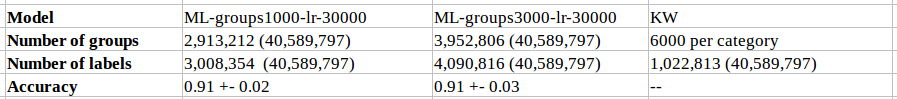
\includegraphics[width=1.0\textwidth]{fig/t-results} 
\end{figure}
}

\frame{
\frametitle{ Results per category: the best and the worst }

\begin{figure}
    \centering
    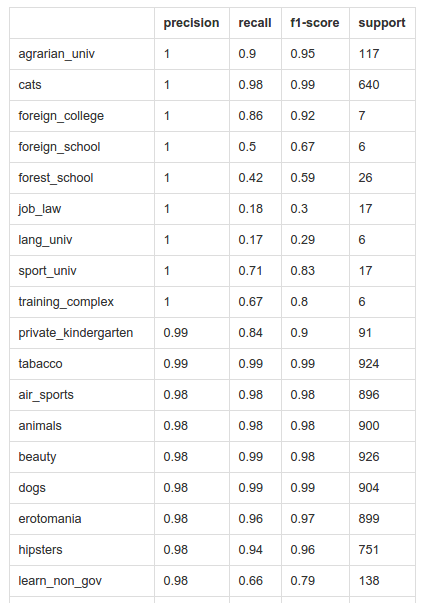
\includegraphics[width=0.5\textwidth]{fig/t-best}
    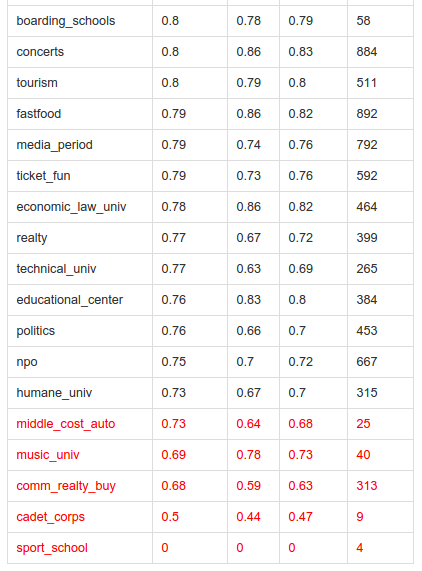
\includegraphics[width=0.49\textwidth]{fig/t-worst} 
\end{figure}
}


\frame{
\frametitle{ Top 30 interests on FB and VK }

\begin{figure}
    \centering
    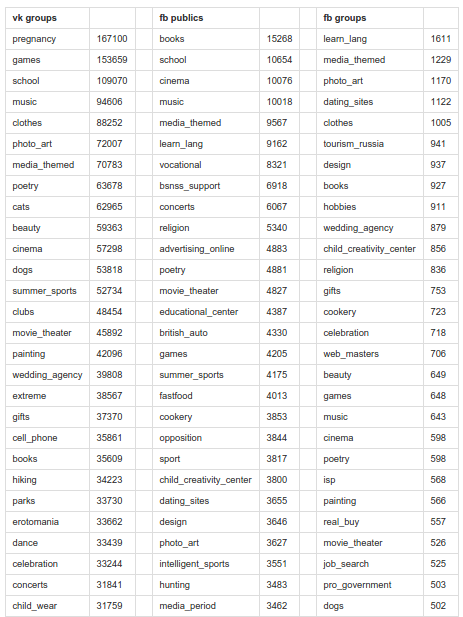
\includegraphics[width=0.6\textwidth]{fig/t-top30-interests} 
\end{figure}
}

\frame{
\frametitle{ Intersection of the top 30 interests on FB and VK }

\begin{figure}
    \centering
    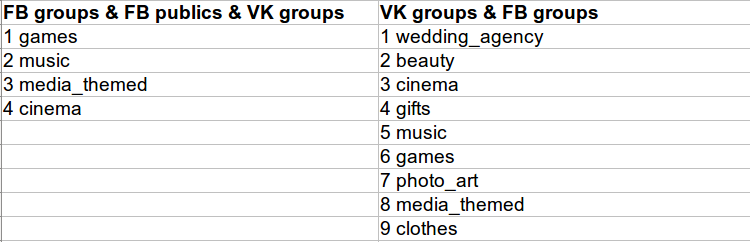
\includegraphics[width=1.0\textwidth]{fig/t-top30-intersection} 
\end{figure}

}

\frame{
\frametitle{ Interests co-occurrences  }

\begin{figure}
    \centering
    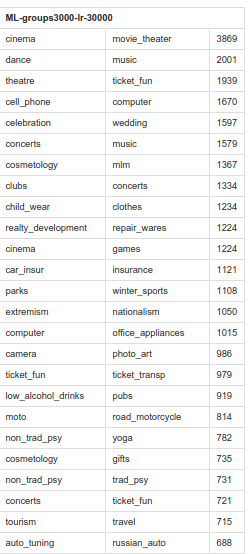
\includegraphics[width=0.4\textwidth]{fig/t-coocur} 
\end{figure}

}


\section[User Matching]{VK-FB User Matching}
\subsection{}

\frame{
\frametitle{ Problem }

\textit{Joint work with Dmitry Babaev and Segei Objedkov.}

\begin{block}{Motivation}

\begin{itemize}
  \item \textbf{\alert{input}}: a user profile of one social network
  \item \textbf{\alert{output}}: profile of the same person in another social network
  \item immediate applications in marketing, search, security, etc. 
\end{itemize}
\end{block}


\begin{block}{Contribution}
\begin{itemize}
  \item user identity resolution approach
  \item precision of 0.98 and recall of 0.54
  \item the method is computationally effective and easily parallelizable
\end{itemize} 
\end{block}
}


\frame{
\frametitle{ Dataset }

\begin{table}
\begin{tabular}{|l|r|r|} \hline
 & VK & Facebook \\ \hline
Number of users in our dataset & 89,561,085 & 2,903,144 \\ 
Number  of users in Russia~\footnote{According to comScore and \url{http://vk.com/about}}  & 100,000,000 & 13,000,000 \\ 
User overlap & 29\% & 88\% \\ \hline
%Average number of friends  & 48 $\pm$ 189  & 72 $\pm$ 232 \\ \hline % 136 % 72 $\pm$ 232 61 $\pm$ 194
\end{tabular}
\label{tab:stat}
\end{table}

\begin{itemize}
  \item \textbf{training set}: 92,488 matched FB-VK profiles 
\end{itemize}
}


\frame{
\frametitle{Profile matching algorithm }

\begin{enumerate}
\item \textbf{Candidate generation}. For each VK profile we retrieve a set of FB profiles with similar first and second names. 
\item \textbf{Candidate ranking}. The candidates are ranked according to similarity of their friends.
\item \textbf{Selection of the best candidate}. The goal of the final step is to select the best match from the list of candidates.
\end{enumerate}
}

\frame{
\frametitle{Candidate generation}
\begin{itemize}
  \item Retrieve FB users with names similar to the input VK profile.
  \item Two names are similar if the first letters are the same and the edit distance between names $\le$ 2.
  \item  Levenshtein Automata for fuzzy match between a VK user name and all FB user names
  \item  Automatically extracted dictionary of name synonyms:
  \begin{itemize}
    \item ``Alexander'', ``Sasha'', ``Sanya'', ``Sanek'', etc.
  \end{itemize}
\end{itemize}

}

\frame{

\frametitle{Candidate ranking}
\begin{itemize}
\item The higher the number of friends with similar names in
VK and FB profiles, the greater the similarity of these profiles.
\item  Two friends are considered to be similar if:

\begin{itemize}
\item First two letters of their last names match
\item \textbf{Similarity between first/last names} $sim_s$ are greater than thresholds $\alpha, \beta$:
$$ 
sim_{s}(s_i,  s_j) =  1-  \frac{lev(s_i, s_j)}{\max(|s_i|, |s_j|)},
$$

\end{itemize}
\item Contribution of each friend to \textbf{similarity $sim_p$ of two profiles} $p_{vk}$ and $p_{fb}$ is inverse of name expectation frequency:  
$$
sim_p (p_{vk}, p_{fb}) = \sum_{ j : sim_s(s^f_i,s^f_j) > \alpha \wedge sim_s(s^s_i, s^s_j) > \beta }  \min (1, \frac{N}{ |s^f_j| \cdot |s^s_j|  }).
$$

Here $s^f_i$ and $s^s_i$ are first and second names of a VK profile, correspondingly, while $s^f_j$ and $s^s_j$ refer to a FB profile.%, $N$ is the number of Facebook profiles, $|s^f_j|$ and $|s^s_j|$ are frequencies of respectively first and second names on Facebook.
 
\end{itemize}

}


\frame{
\frametitle{Best candidate selection}
\begin{itemize}
\item FB candidates are ranked according to similarity $sim_p$ to an input profile $p_{vk}$

\item The best candidate $p_{fb}$ should pass two thresholds to match:

\begin{itemize}

\item its score should be higher than the \textit{score threshold} $\gamma$:
$$
sim_p(p_{vk},p_{fb}) > \gamma.
$$ 

\item either the only candidate or score ratio between it and the next best candidate $p'_{fb}$ should be higher than the \textit{ratio threshold} $\delta$:
$$
\frac{sim_p(p_{vk},p_{fb})}{sim_p(p_{vk},p'_{fb})} > \delta.
$$
\end{itemize}
\end{itemize}
}


\frame{
\frametitle{Results}

\begin{figure}
\centering
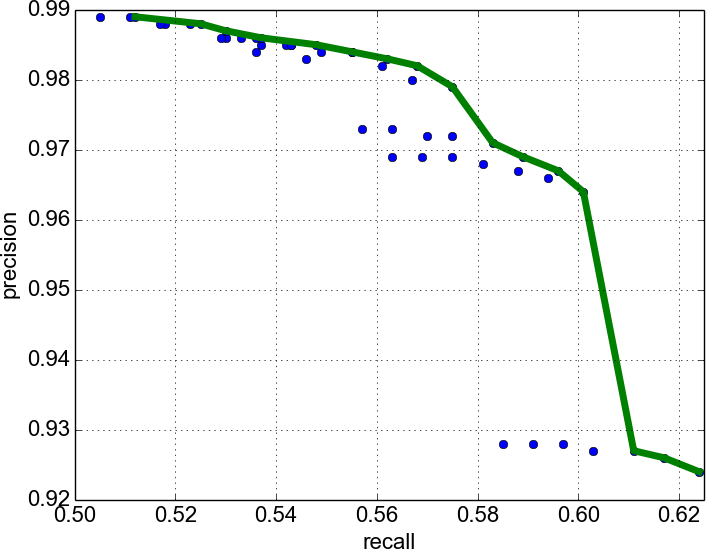
\includegraphics[width=0.5\textwidth]{fig/pr-new-all}
\caption{Precision-recall plot of the matching method. The bold line denotes the best precision at given recall. }
\label{fig:pr}
\end{figure}

}

\frame{
\frametitle{Results: matching VK and FB profiles}

\begin{table}

\centering
%\caption{Matching VKontakte and Facebook profiles: parameters of the method and results. }
\begin{tabular}{|l|l|} \hline
First name threshold, $\alpha$ & 0.8 \\ 
Second name threshold, $\beta$ & 0.6 \\ 
Profile score threshold, $\gamma$ & 3 \\ 
Profile ratio threshold, $\delta$ & 5 \\ \hline \hline 
Number of matched profiles & 644,334 (22\%) \\ 
Expected precision & 0.98 \\ 
Expected recall & 0.54 \\ \hline

\end{tabular}
\label{tab:results}
\end{table}

}


\section[Sentiment Index]{Sentiment Index of the Russian Speaking Facebook}

\frame{
\frametitle{ Statistics of the Facebook corpus 2013}

\begin{figure}
\centering
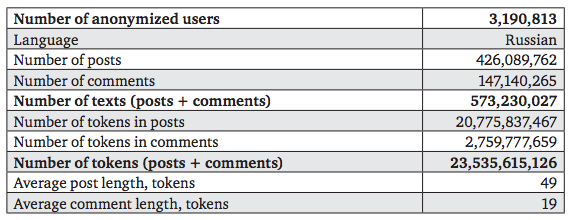
\includegraphics[width=0.99\textwidth]{fig/fb-corpus}
\caption{Statistics of the Facebook corpus. }
\end{figure}

}


\frame{
\frametitle{ Most frequent positive and negative adjectives in the Facebook corpus}

\begin{figure}
\centering
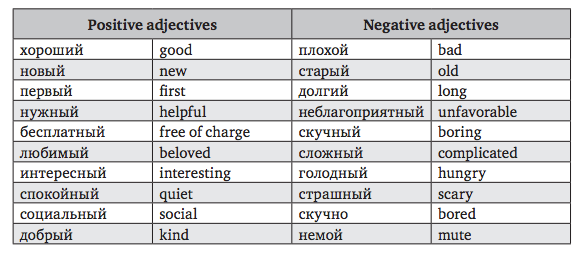
\includegraphics[width=0.99\textwidth]{fig/fb-voc}
\end{figure}
}


\frame{
\frametitle{  Performance of the dictionary-based sentiment classification
approach, as compared to other methods (ROMIP-2012)}

\begin{figure}
\centering
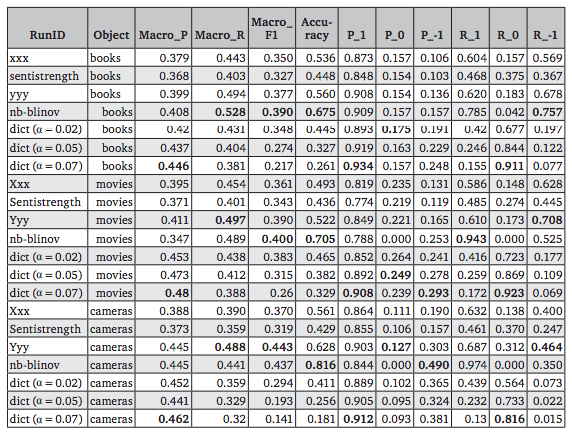
\includegraphics[width=0.99\textwidth]{fig/fb-method}
\end{figure}
}



\frame{
\frametitle{ Results of the social sentiment index calculation}

\begin{figure}
\centering
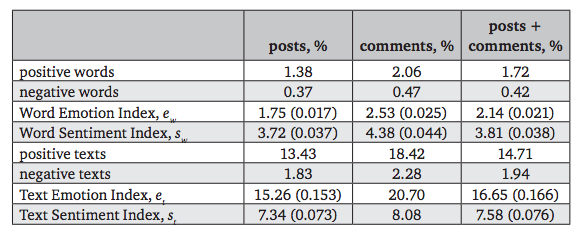
\includegraphics[width=0.99\textwidth]{fig/fb-results}
\end{figure}
}



\frame{
\frametitle{ Results of the social sentiment index calculation }

\begin{figure}
\centering
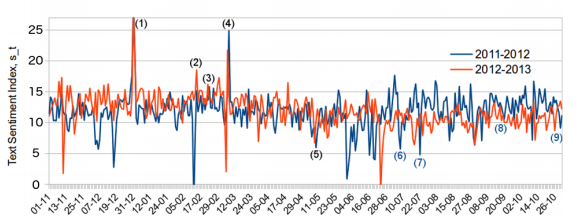
\includegraphics[width=0.99\textwidth]{fig/fb-index}


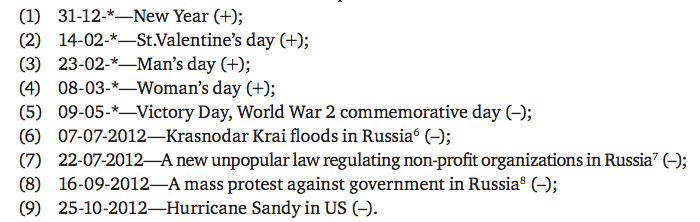
\includegraphics[width=0.65\textwidth]{fig/fb-index-dates}
\end{figure}
}





\section[Other tasks]{Other Tasks}
\subsection{}

\frame{
\frametitle{ Much more fun stuff can be done with the FB/VK data }

\begin{itemize}

  \item \textbf{Neologism Detection}
  \begin{itemize}
  	\item Build frequency dictionary of posts and comments.
  	\item Filter out dictionary words and grammatical errors. 
  	\item Interpret most frequent non-dictionary words linguistically. 
  \end{itemize}

  \item \textbf{User Age \& Region Detection}
  \begin{itemize}
    \item Tell me who are your friends, and I will say who you are.
    \item Most frequent age/region of friends.
    \item Reject users with high variation of age/region among friends.
    \item Up to 85-90\% of accuracy. 
  \end{itemize}
   
  \item \textbf{User Income Detection}
  \begin{itemize}
    \item Transfer learning: target variable is not present in SNs.
    \item Training a model on a set of users with known income.
    \item Applying the model on the social network profiles. 
  \end{itemize} 
  
\end{itemize}

}


\frame{
\frametitle{ }
\textbf{\Huge Thank you! Questions?}
}


%unsrt,alpha,abbrv,acm,apalike
\bibliographystyle{apalike}
\bibliography{biblio2}

\end{document}
